%%% Preamble
\documentclass[paper=a4, fontsize=11pt]{report}
\usepackage[utf8]{inputenc}
\usepackage[T1]{fontenc}
\usepackage{fourier}
\usepackage[french]{babel}
\usepackage[protrusion=true,expansion=true]{microtype}	
\usepackage{amsmath,amsfonts,amsthm} % Math packages
\usepackage[pdftex]{graphicx}	
\usepackage{url}
\usepackage{pdfpages}
\usepackage{todonotes}
\usepackage[a4paper, body={17cm,26cm}]{geometry}
\usepackage{float}
\usepackage{framed}
\usepackage[toc,page]{appendix} 
\usepackage{multicol}
\usepackage{colortbl}

%%% Custom sectioning
\usepackage{sectsty}
\allsectionsfont{  \normalfont\scshape}
%\allsectionsfont{\centering \normalfont\scshape}

%%% Custom headers/footers (fancyhdr package)
\usepackage{fancyhdr}
\pagestyle{fancyplain}
\fancyhead{}											% No page header
\fancyfoot[L]{}											% Empty 
\fancyfoot[C]{}											% Empty
\fancyfoot[R]{\thepage}									% Pagenumbering
\renewcommand{\headrulewidth}{0pt}			% Remove header underlines
\renewcommand{\footrulewidth}{0pt}				% Remove footer underlines
\setlength{\headheight}{13.6pt}


%%% Equation and float numbering
\numberwithin{equation}{section}		% Equationnumbering: section.eq#
\numberwithin{figure}{section}			% Figurenumbering: section.fig#
\numberwithin{table}{section}				% Tablenumbering: section.tab#


%%% Define new commands
\newcommand{\horrule}[1]{\rule{\linewidth}{#1}} 	% Horizontal rule
\renewcommand{\bf}[1]{\textbf{#1}}
\renewcommand{\it}[1]{\textit{#1}}

\newcommand{\Todo}[1]{\todo[inline]{#1}}
\renewcommand{\thesection}{\thepart .\arabic{section}}

\usepackage{cases}
\usepackage{color}
\usepackage{xcolor}
\usepackage{relsize}

\usepackage{caption}
\DeclareCaptionFont{white}{\color{white}}
\DeclareCaptionFormat{listing}{\colorbox{gray}{\parbox{\textwidth}{#1#2#3}}}
\captionsetup[lstlisting]{format=listing,labelfont=white,textfont=white}

\usepackage[numbered]{mcode}

\lstset{breaklines=true,columns=fullflexible}
\colorlet{shadecolor}{black!10}



\delimitershortfall-1sp
\newcommand\abs[1]{\left|#1\right|}




%%% Begin document
\begin{document}
\includepdf[pages={1}]{title.pdf}

\tableofcontents
\listoftodos

\newpage

%%%%%%%%%%%%%%%%%%%%%%%%%%%%%%%%%%%%%%%%%%%%%%%%%%%%%%%%%%%%%%%%%%%%%%%%%%%%%%%%%%%%%%%%%%%%%%%%%%%%%%%%%%%%%%%%%%%%%%%%%%%
%%%%%%%%%%%%%%%%%%%%%%%%%%%%%%%%%%%%%%%%%%%%%%%%%%%%%%%%%%%%%%%%%%%%%%%%%%%%%%%%%%%%%%%%%%%%%%%%%%%%%%%%%%%%%%%%%%%%%%%%%%%
%%%%%%%%%%%%%%%%%%%%%%%%%%%%%%%%%%%%%%%%%%%%%%%%%%%%%%%%%%%%%%%%%%%%%%%%%%%%%%%%%%%%%%%%%%%%%%%%%%%%%%%%%%%%%%%%%%%%%%%%%%%
\part{\'Etude des problèmes soumis par les responsables}

\section{Introduction}
Cette section traite de la résolution des problèmes soumis par les différents acteurs de l'entreprise. Chaque sous-section aborde un problème et tente de proposer une solution optimale plausible pour ce dernier.

%%%%%%%%%%%%%%%%%%%%%%%%%%%%%%%%%%%%%%%%%%%%%%%%%%%%%%%% NOTATIONS %%%%%%%%%%%%%%%%%%%%%%%%%%%%%%%%%%%%%%%%%%%%%%%%%%%%%%%%

\begin{shaded}
\vspace{-0.5cm}

\subsection*{Notations}
Dans le document suivant, nous allons utiliser : 
$A$, $B$, $C$, $D$, $E$ et $F$ pour désigner les différents produits $P_i$. Les quantités respectives $q_i$ seront désignées par $q_A$, $q_B$, $q_C$, $q_D$, $q_E$ et $q_F$. Le prix de vente du produit $P_i$ sera noté $p_i$. Le coût de production du produit $P_i$ sera noté $c_i$, le coût de production comprends le coût des matières premières et le coût de fabrication dû aux machines.\\

Le vecteur des quantités $(q_A$, $q_B$, $q_C$, $q_D$, $q_E$, $q_F)$ sera noté $Q$ dans la suite du rapport.
\end{shaded}

%%%%%%%%CONTRAINTES GENERALES%%%%%%%%%%%%%%%%%%%%%%%%%%%%%%%%%
\section{Contraintes Générales}

Afin de modéliser la production de l'atelier, il est nécessaire de définir plusieurs contraintes établies à la suite de l'analyse des conditions de production.

\subsection{Contraintes sur la quantité}

La quantité de chaque produit doit être supérieure à 0. Les produits $A$ et $B$ doivent être au moins fabriqués en 5 exemplaires par semaine.

Ceci se traduit par les contraintes de domaines suivantes : 

\begin{equation}
q_A \geq 5, \quad q_B \geq 5, \quad q_C \geq 0, \quad q_D \geq 0, \quad q_E \geq 0, \quad q_F \geq 0 
\label{ctr_quantite}
\end{equation} 

\subsection{Contraintes sur le stockage}
Les contraintes de stockage imposent des quantités sur les matières premières. L'entreprise ne peut stocker qu'au maximum 350 unités de la matière première 1, 620 de la matière première 2 et 485 de la matière première 3. Sachant que l'on connaît le nombre de matières premières nécessaires à la fabrication de chaque produit, on obtient les trois contraintes suivantes :  

\begin{equation}
  \left\{
    \begin{aligned}
q_A + 2 q_B + q_C + 5q_D + 2q_F \quad & \leq & 350 \\
2q_A + 2q_B + q_C + q_D + q_E \quad & \leq & 620 \\
q_A + 3 q_C + 2q_D + 2q_E \quad & \leq & 485 
    \end{aligned}
  \right.
\label{ctr_stockage}
\end{equation}

\subsection{Contraintes sur le temps de travail}

L'entreprise travaille en 2 huit, 5 jours sur 7. Ceci correspond à 80 heures ou encore $4\:800$ minutes par semaine. Par exemple, la machine 1 est utilisée pendant 8 minutes afin de fabriquer un produit A, 15 minutes pour un produit B, 5 minutes pour un produit D et 10 minutes pour un produit F.

Ceci permet d'établir les contraintes sur le temps d'utilisation des machines (7 machines au total) : 

\begin{equation}
  \left\{
    \begin{aligned}
8q_A + 15q_B +  5q_D + 10q_F \quad & \leq & 4800 & \quad \text{(machine 1)} \\
7q_A + 12q_B + 2q_C  + 15q_D + 7q_E  + 12q_F \quad & \leq & 4800 & \quad \text{(machine 2)} \\
8q_A +   q_B + 11q_C + 10q_E + 25q_F \quad & \leq & 4800 & \quad \text{(machine 3)} \\
2q_A + 10q_B + 5q_C  +  4q_D + 13q_E + 7q_F  \quad & \leq & 4800 & \quad \text{(machine 4)} \\
5q_A + 8q_C  +  7q_D + 10q_E + 25q_F \quad & \leq & 4800 & \quad \text{(machine 5)} \\
5q_A +  5q_B + 3q_C  + 12q_D + 8q_E  + 6q_F  \quad & \leq & 4800 & \quad \text{(machine 6)} \\
5q_A +  3q_B + 5q_C  + 8q_D  + 7q_F  \quad & \leq & 4800 & \quad \text{(machine 7)} 
    \end{aligned}
  \right.
\label{tps_travail}
\end{equation}

\subsection{Bilan des contraintes}

Ces contraintes seront utilisées afin de calculer les solutions de production respectant les objectifs de chaque responsable. Pour chaque objectif, il s'agira alors de minimiser une fonction $f$ telle que :

\begin{equation}
  min(f^T(Q)) \quad \text{tel que :} \quad \\
   \left\{
    \begin{aligned}
A.Q \quad & \leq & b \\
lb \quad & \leq & x \\
    \end{aligned}
  \right.
\end{equation}

\[ \text{Avec : } \quad A = \begin{bmatrix}
1 & 2 & 1 & 5 & 0 & 2 \\ 
2 & 2 & 1 & 2 & 2 & 1 \\ 
1 & 0 & 3 & 2 & 2 & 0 \\ 
8 & 15 & 0 & 5 & 0 & 10 \\ 
7 & 12 & 2 & 15 & 7 & 12 \\ 
8 & 1 & 11 & 0 & 10 & 25 \\ 
2 & 10 & 5 & 4 & 13 & 7 \\ 
5 & 0 & 8 & 7 & 10 & 25 \\ 
5 & 5 & 3 & 12 & 8 & 6 \\ 
5 & 3 & 5 & 8 & 0 & 7 
\end{bmatrix} \quad \quad
b = \begin{bmatrix}
350 \\ 
620 \\ 
485 \\ 
4800 \\ 
4800 \\ 
4800 \\ 
4800 \\ 
4800 \\ 
4800 \\ 
4800
\end{bmatrix} \quad \quad
lb = \begin{bmatrix}
5 \\
5 \\
0 \\
0 \\
0 \\
0
\end{bmatrix} 
  \]

Ainsi, pour reproduire les résultats obtenus dans ce rapport, il suffira d'utiliser la fonction \bf{linprog($f$, $A$, $b$, [], [], $lb$)} de \textit{Matlab}, où $f$ est un vecteur, dont les composants sont les coefficients de la fonction à minimiser.

\begin{shaded}
\vspace{-0.5cm}

\subsection*{Notes sur les contraintes}
Dans la suite du rapport, l'ensemble des responsables utilisera les équations \eqref{ctr_quantite}, \eqref{ctr_stockage} et \eqref{tps_travail}. \\

Des contraintes supplémentaires peuvent être également ajoutées au cas par cas. Dans ce cas, elles seront explicitement précisées dans le texte.
\end{shaded}

%%%%%%%%%%%%%%%%%%%%%%%%%%%%%%%%%%%%%%%%%%%%%%%%%%%%%%%% COMPTABLE %%%%%%%%%%%%%%%%%%%%%%%%%%%%%%%%%%%%%%%%%%%%%%%%%%%%%%%%
\section{Comptable}
\bf{Problème soumis :}

Le comptable souhaite maximiser les bénéfices de l'entreprise.\\

\bf{Solution proposée :}

Nous avons cherché à optimiser la production afin de maximiser le bénéfice de l'entreprise, qui correspond à la différence entre le prix de vente et le coût de production. La fonction à maximiser corrrespond donc à la suivante :

\[f(Q) = (\sum_i q_i \times p_i ) - (\sum_i q_i \times c_i) \quad \text{  avec } \, Q, \, \text{ vecteur des quantités } \, q_i \]

\bf{Résultat :}

Les quantités optimales de produits à fabriquer chaque semaine correspondent aux valeurs suivantes :

\begin{center}
\begin{tabular}{cccccc}
\hline
$q_A$ & $q_B$ & $q_C$ & $q_D$ & $q_E$ & $q_F$ \\
\hline
5 & 18 & 0 & 0 & 240 & 93,67 \\
\hline
\end{tabular}
\end{center}

Ce résultat se comprend plus facilement si l'on regarde la rentabilité (bénéfice en euros pour une unité fabriquée) de chaque produit, présentée ci-dessous :

\begin{center}
\begin{tabular}{cccccc}
\hline
$r_A$ & $r_B$ & $r_C$ & $r_D$ & $r_E$ & $r_F$ \\
\hline
5,83 & 11,61 & 12,16 & 1,3 & 31,65 & 27,48 \\
\hline
\end{tabular}
\end{center}

Dans ce cas, le bénéfice optimal hebdomadaire est de $10\:408\,$€.\\

Nous pouvons remarquer que le produit E est le plus rentable, suivi du produit F, C, B, A et enfin D. De ce fait, il est plus intéressant de favoriser la production des produits en suivant cet ordre et ainsi de favoriser le produit E, à l'inverse du produit D. Cependant, nous pouvons également remarquer que le produit C, qui possède une meilleure rentabilité que le produit B, est pourtant produit en moins grande quantité que ce dernier. Cela s'explique par le fait que les produits les plus rentables (E et F) utilisent la plupart des matières premières. Le produit C utilisant les mêmes matières premières que E et F, le produit B sera favorisé à C malgré une rentabilité inférieure.

%%%%%%%%%%%%%%%%%%%%%%%%%%%%%%%%%%%%%%%%%%%%%%%%%%%%%%%% RESP ATELIER %%%%%%%%%%%%%%%%%%%%%%%%%%%%%%%%%%%%%%%%%%%%%%%%%%%%%%%%

\section{Responsable d'atelier}
\bf{Problème soumis :}

Le responsable de l'atelier souhaite maximiser la quantité totale de produits fabriqués. De ce fait, la fonction à maximiser ne devra pas favoriser un type de produit par rapport à un autre, seul le nombre total de produits fabrqués étant important.\\

\bf{Solution proposée :}

Nous cherchons à maximiser l'équation (en tenant compte des contraintes générales) suivante :

\[f(Q) = \sum_i q_i \quad \text{  avec } \, Q, \, \text{ vecteur des quantités } \, q_i \]

\bf{Résultat :}

Les quantités optimales à produire, selon le responsable atelier, sont les suivantes :

\begin{center}
\begin{tabular}{cccccc}
\hline 
$q_A$ & $q_B$ & $q_C$ & $q_D$ & $q_E$ & $q_F$ \\ 
\hline 
5,00 & 54.64 & 38,85 & 0,00 & 181,71 & 98,43 \\ 
\hline 
\end{tabular} 
\end{center}

Nous constatons donc qu'il est préférable d'éviter de fabriquer des produits D si l'on souhaite maximiser le nombre de produits à fabriquer. Cependant, ceci n'est pas une solution qui sera compatible avec les autres responsables. En effet, il y a un déséquilibre important entre la production des produits $A$ et $E$, ce qui ne conviendra pas au responsable commercial.\\

Cette étude nous permet de trouver la quantité maximale de produits qui peut être produite par l'entreprise, soit :
\[ Q_{max} = 378,6 \text{ produits}\]

Cette limite supérieure présente l'intérêt de proposer un intervale de recherche pour d'autres études.


%%%%%%%%%%%%%%%%%%%%%%%%%%%%%%%%%%%%%%%%%%%%%%%%%%%%%%%% RESP DES STOCK %%%%%%%%%%%%%%%%%%%%%%%%%%%%%%%%%%%%%%%%%%%%%%%%%%%%%%%%
\section{Responsable des stocks}
\bf{Problème soumis :}

Le responsable des stocks souhaite quant à lui minimiser la quantité de matières stockées (qu'elle soit brute ou transformée).\\

Ainsi, nous devons minimiser la quantité de produits stockés (c'est-à-dire minimiser $q_A + q_B + q_C + q_D + q_E + q_F$), ainsi que les matières premières stockées (soit $4q_A + 4q_B + 5q_C + 9q_D + 4q_E + 3q_F$).
\\

\bf{Solution proposée :}

La fonction à minimiser est la suivante : 

\[ f(Q) = 5q_A + 5q_B + 6q_C + 10q_D + 5q_E + 4q_F \]

Cependant, sans contrainte supplémentaire, nous sommes dans le cas irréaliste où l'on pourrait diminuer d'autant que l'on souhaite le nombre de produits fabriqués par l'entreprise. Il faut donc ajouter une contrainte, qui peut être une contrainte sur un nombre minimal de produits à fabriquer, ou bien sur le bénéfice minimal souhaité.
Pour l'étude, un nombre minimal de produits à fabriquer a été fixé. Nous avons fait varier ce nombre pour voir s'il n'y a pas un point idéal sur les courbes ci-dessous, qui représenterait un compromis acceptable pour le responsable des stocks.\\

Il est important de noter que les courbes suivantes ont été obtenues en faisant varier uniquement la contrainte sur le nombre de produits minimum à fabriquer.\\

\bf{Résultat :}

\begin{figure}[H]
\caption{Nombre de produits en fonction du stock total \label{figstock}}
\centering
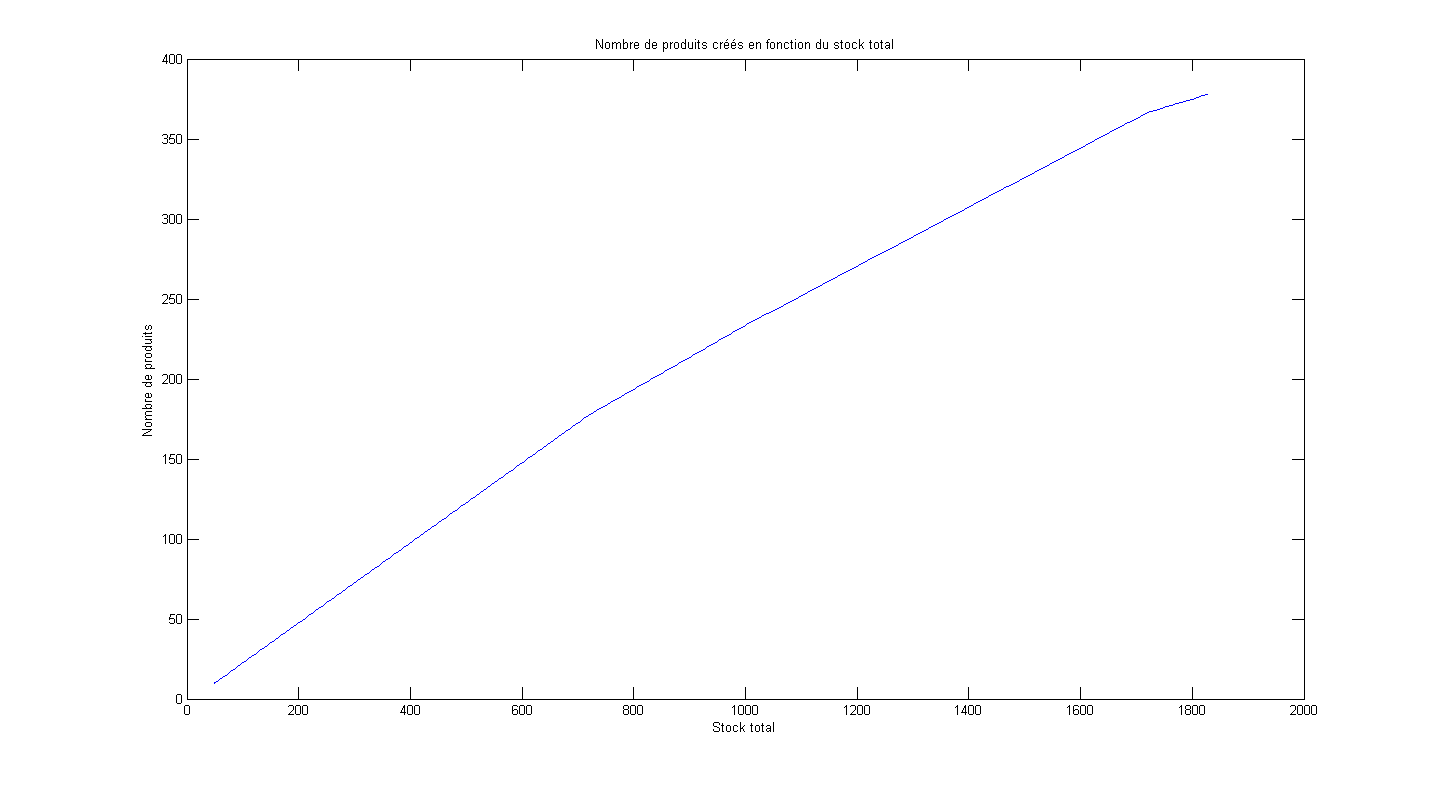
\includegraphics[width=16cm]{figures/nbProduitsFctStockTotal.png}
\end{figure}

\begin{figure}[H]
\caption{Variation du coefficient de la courbe de la figure \ref{figstock}}
\centering
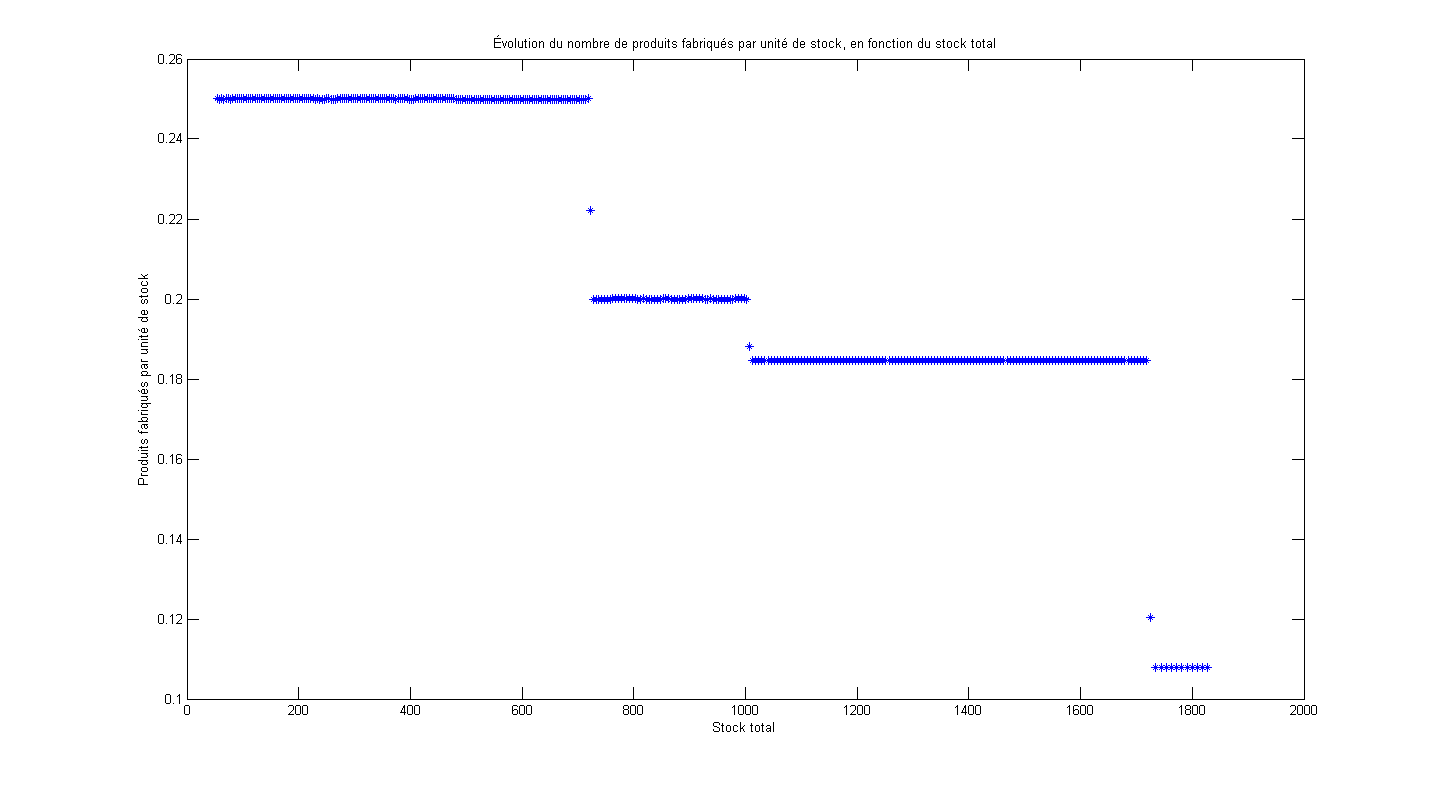
\includegraphics[width=16cm]{figures/nbProduitsFctStockTotal_Coeff.png}
\end{figure}

\begin{figure}[H]
\caption{Bénéfice réalisé en fonction du stock total \label{figben}}
\centering
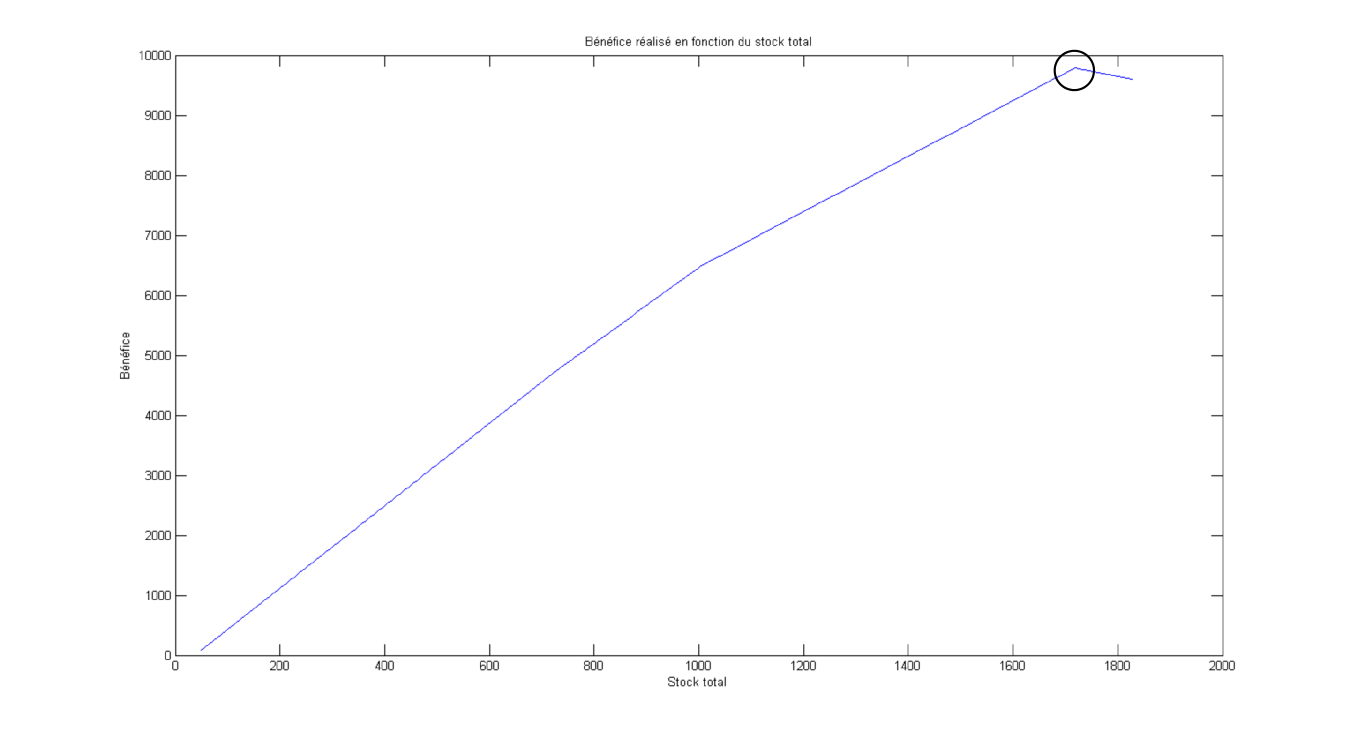
\includegraphics[width=16cm]{figures/BenefFctStockTotal.png}
\end{figure}

\begin{figure}[H]
\caption{Variation du coefficient de la courbe de la figure \ref{figben}}
\centering
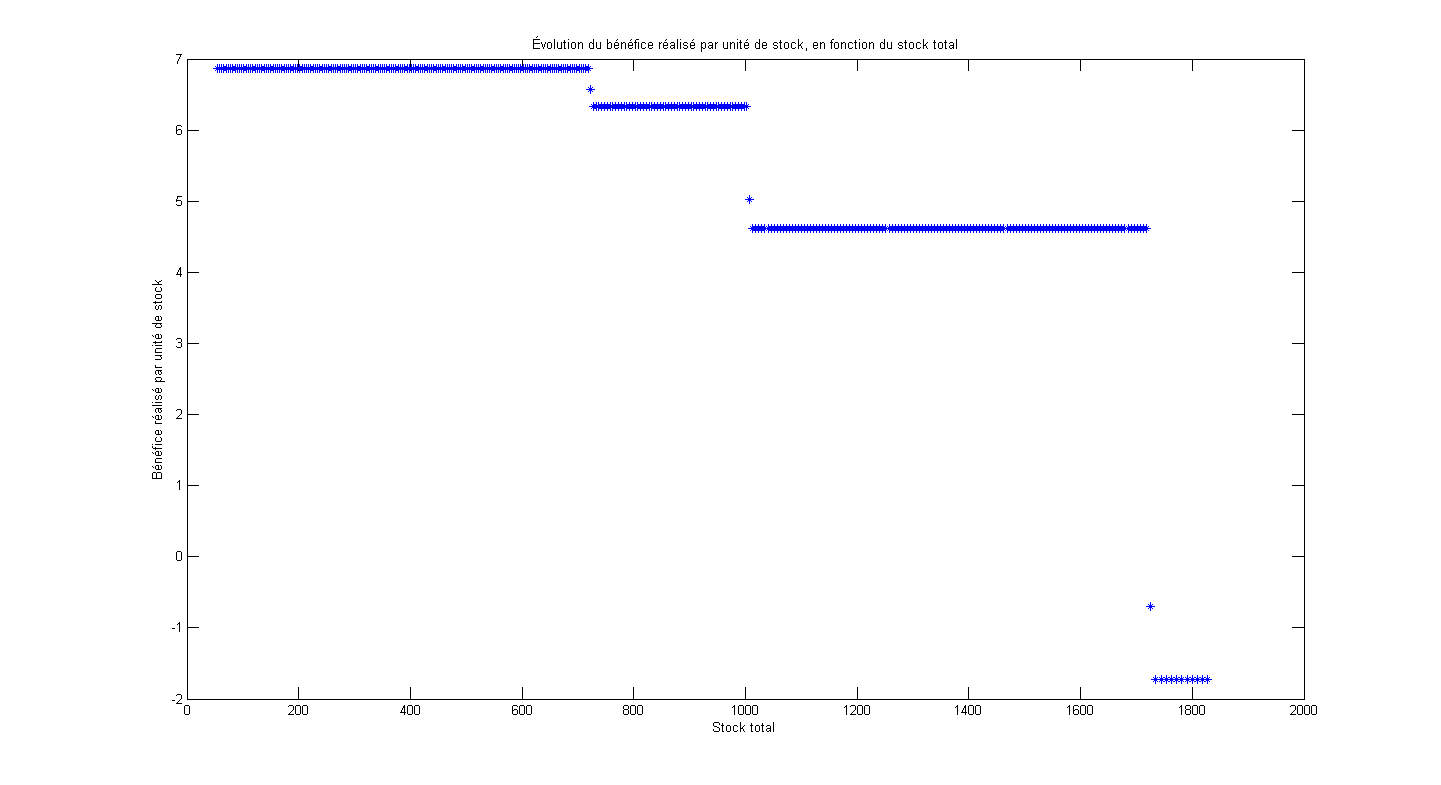
\includegraphics[width=16cm]{figures/BenefFctStockTotal_Coeff.png}
\end{figure}

Les figures nous montrent que pour une production réaliste de produits ($> 200$), la rentabilité par produit chute à partir de 1 003 unités de stocks, soit une production de 243 produits dont Matlab nous donne la répartition suivante :

\begin{center}
\begin{tabular}{cccccc}
\hline 
$q_A$ & $q_B$ & $q_C$ & $q_D$ & $q_E$ & $q_F$ \\ 
\hline 
5,00 & 5,00 & 0,00 & 0,00 & 56,5 & 167,5 \\ 
\hline 
\end{tabular} 
\end{center}

Un autre point peut également être considéré comme une répartition optimale des stocks. Il s'agit du dernier point où nous constatons une variation brutale du coefficient directeur des courbes (qui correspond à 1 717 unités de stocks, 366 produits, ou encore un bénéfice de 9 786 €). À cet endroit, nous obtenons la répartition des quantités fabriquées suivante :

\begin{center}
\begin{tabular}{cccccc}
\hline 
$q_A$ & $q_B$ & $q_C$ & $q_D$ & $q_E$ & $q_F$ \\ 
\hline 
5.00 & 53,23 & 0,00 & 0,00 & 172,50 & 119,27 \\ 
\hline 
\end{tabular} 
\end{center}

Le second choix a l'inconvénient d'avoir un ratio bénéfice/stockage moins élevé mais présente l'avantage d'être mieux en accord avec le nombre de produits à produire vis-à-vis des autres responsables. Cependant, nous choisirons ce second choix afin de ne pas trop pénaliser les critères des autres responsables.

%%%%%%%%%%%%%%%%%%%%%%%%%%%%%%%%%%%%%%%%%%%%%%%%%%%%%%%% RESP COMMERCIAL %%%%%%%%%%%%%%%%%%%%%%%%%%%%%%%%%%%%%%%%%%%%%%%%%%%%%%%%
\section{Responsable commercial}
\bf{Problème soumis :}

Le responsable commercial souhaite équilibrer la quantité fabriquée des produits A et E.\\

\bf{Solution proposée :}

Afin de trouver une solution optimale pour le responsable commercial, nous devons maximiser les bénéfices tout en ajoutant une contrainte supplémentaire au modèle général. Cette contrainte doit permettre d'équilibrer la production des produits A et E, qui est la priorité du responsable commercial. Cette contrainte se traduit par l'égalité suivante : $q_A = q_E$. \\

Nous souhaitons donc minimiser l'écart entre $q_A$ et $q_E$, tel que :

\[ \abs{q_A - q_E} \leq \epsilon \] 

Pour un écart nul entre les quantités de A et E produites, nous avons les quantités hebdomadaires suivante :
\begin{center}
\begin{tabular}{cccccc}
\hline
$q_A$ & $q_B$ & $q_C$ & $q_D$ & $q_E$ & $q_F$ \\
\hline
119.08 & 6.91 & 42.58 & 0.00 & 119.08 & 87.24 \\
\hline
\end{tabular}
\end{center}

Nous pouvons remarquer de nouveau que le produit D ne semble pas rentable car l'étude conclue qu'il serait optimal de ne plus le produire. Nous remarquons également que l’évolution de $e$ tend à favoriser la production du produit E plutôt que le produit A.

%%%%%%%%%%%%%%%%%%%%%%%%%%%%%%%%%%%%%%%%%%%%%%%%%%%%%%%% RESP DU PERSONNEL %%%%%%%%%%%%%%%%%%%%%%%%%%%%%%%%%%%%%%%%%%%%%%%%%%%%%%%%
\section{Responsable du personnel}
\bf{Problème soumis :}

Le responsable du personnel souhaite utiliser le moins possible la machine 4.\\

\bf{Solution proposée :}

La première solution qui nous vient à l’esprit serait de minimiser la fonction suivante : \[f(Q) = 2q_A + 10q_B + 5q_C + 4q_D + 13q_E + 7q_F\]

Cette fonction traduit l'utilisation de la machine 4 en fonction des produits fabriqués. Cependant, les résultats que nous obtenons en ne prenant en compte que cette équation ne sont pas satisfaisants, car nous nous retrouvions à produire 5 unités de A et B et 0 des autres produits. Ce résultat est mathématiquement juste au vu des contraintes que nous avions précisées, mais ne suffit pas pour assurer une rentabilité à l’entreprise. Pour trouver une solution plus juste, nous allons prendre en compte une certaine quantité d’unités minimales à produire. \\

\bf{Contraintes supplémentaires :}

Nous reprenons donc les résultats obtenus par le responsable d’atelier, et en faisant varier les différentes quantités de produits fabriqués selon sa méthode de calcul, nous avons établi un graphique ci-dessous permettant d’évaluer le temps d’utilisation de la machine 4.\\

\begin{figure}[H]
\caption{Temps d'utilisation de la machine 4 en fonction du nombre de produits fabriqués}
\centering
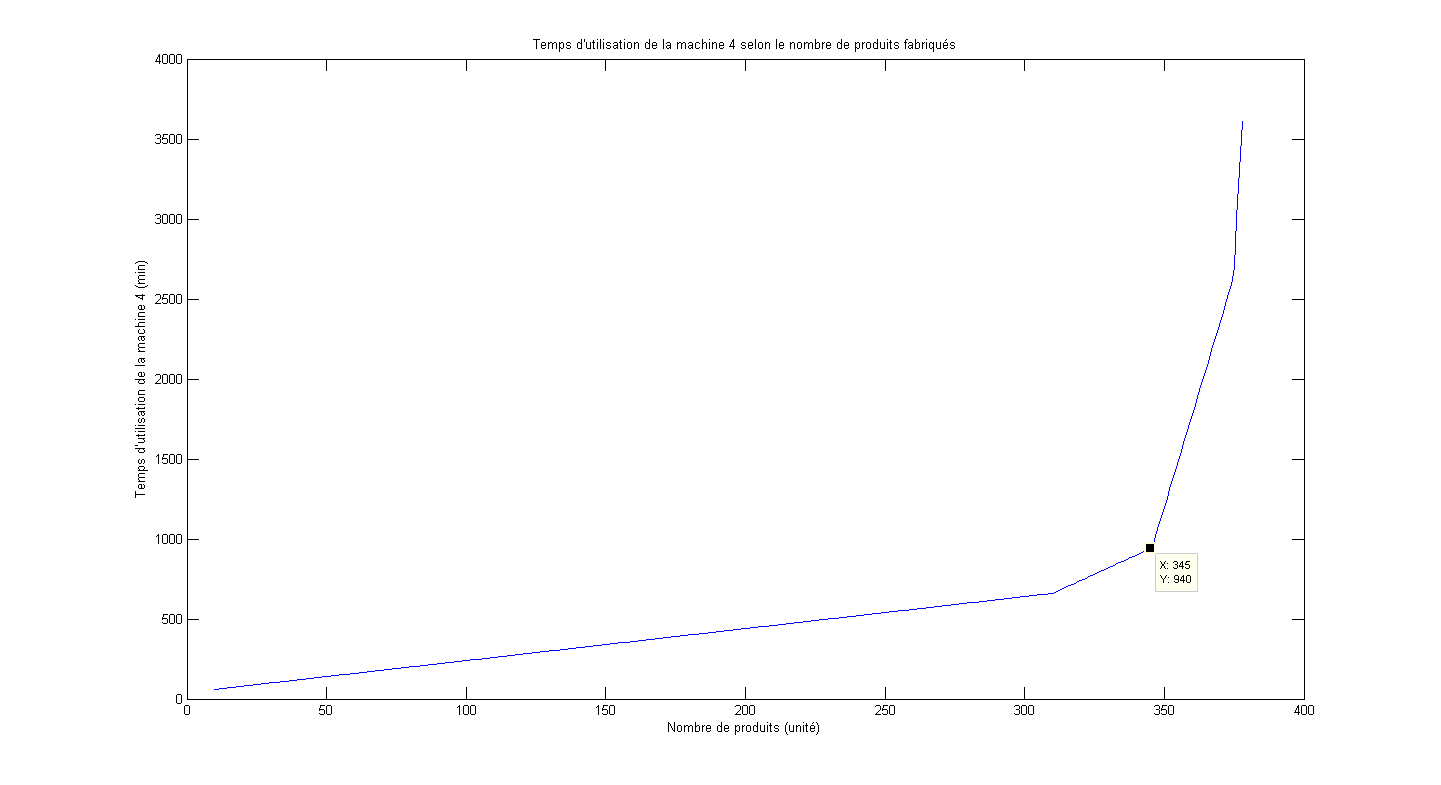
\includegraphics[width=16cm]{figures/graphe-personnel.png}
\end{figure}

Nous constatons très clairement que la pente de la courbe augmente fortement à partir de 345 unités fabriquées, ce qui correspond à 940 minutes de travail pour la machine 4. Au delà de ce seuil, la machine 4 est beaucoup plus utilisée pour chaque unité de produit fabriqué.\\

Nous choisirons donc la limite de 345 unités à produire afin de bénéficier d'un ratio quantité/utilisation de la machine 4 intéressant. La répartition des produits à fabriquer, selon le responsable du personnel, est la suivante : 

\begin{center}
\begin{tabular}{cccccc}
\hline
$q_A$ & $q_B$ & $q_C$ & $q_D$ & $q_E$ & $q_F$ \\
\hline
270.00 & 5.00 & 70.00 & 0.00 & 0.00 & 0.00 \\
\hline
\end{tabular}
\end{center}

\section{Bilan}

Nous pouvons résumer les différents résultats sélectionnés pour chaque responsable dans le tableau ci-dessous. À chaque responsable est également associé un point de mire, qui correspond à son objectif, réalisé grâce à la répartition des produits fabriqués qui a été retenue.


\Todo{problème sur la ligne du responsable des stocks !}
\begin{center}
\begin{tabular}{l|cccccc|cc}
\hline
Responsables & $q_A$ & $q_B$ & $q_C$ & $q_D$ & $q_E$ & $q_F$ & $\sum q_i \quad$ & Point de Mire \\
\hline
Comptable & 5,00 & 18,00 & 0,00 & 0,00 & 240,00 & 93,67 & 356,67 & $10 \:408\,$€\\
Responsable d'atelier & 5,00 & 54,64 & 38,85 & 0,00 & 181,71 & 98,43 & 378,63 & 378,63 produits\\
Responsable des stocks & 5,00 & 53,23 & 0,00 & 0,00 & 172,50 & 119,27 & $1\:717\,$ unités de stocks\\
Responsable commercial & 119,08 & 6,91 & 42,58 & 0,00 & 119,08 & 87,24 & 374,89 & $\abs{q_A - q_E}=0$\\
Responsable personnel & 270,00 & 5,00 & 70,00 & 0,00 & 0,00 & 0,00 & 345,00 & $940\,$ min \\

\hline
\end{tabular}
\end{center}
%%%%%%%%%%%%%%%%%%%%%%%%%%%%%%%%%%%%%%%%%%%%%%%%%%%%%%%%%%%%%%%%%%%%%%%%%%%%%%%%%%%%%%%%%%%%%%%%%%%%%%%%%%%%%%%%%%%%%%%%%%%%%%%%
%%%%%%%%%%%%%%%%%%%%%%%%%%%%%%%%%%%%%%%%%%%%%%%%%%%%%%%% RESP DES STOCK %%%%%%%%%%%%%%%%%%%%%%%%%%%%%%%%%%%%%%%%%%%%%%%%%%%%%%%%
%%%%%%%%%%%%%%%%%%%%%%%%%%%%%%%%%%%%%%%%%%%%%%%%%%%%%%%%%%%%%%%%%%%%%%%%%%%%%%%%%%%%%%%%%%%%%%%%%%%%%%%%%%%%%%%%%%%%%%%%%%%%%%%%
\part{\'Etude du problème soumis par le Responsable de l'entreprise}
\setcounter{section}{0}

\section{Introduction et explication de la démarche}

Nous allons essayer dans cette deuxième partie de satisfaire au mieux les différents responsables. Pour résoudre ce problème, nous allons d'abord établir la matrice avec les points de mire des différents responsables. Ensuite, comme les objectifs des différents responsables sont exprimés dans des unités différentes, il nous faudra normaliser la matrice de gain.

\section{Obtention des points de mire}
Nous calculons dans un premier temps le résultat espéré pour chaque responsable, en fonction du point de mire des autres responsables. Nous obtenons alors le tableau suivant : 

\Todo{Modifier ligne resp stock pour faire avec 1714 : deuxieme sol}
\Todo{Entêtes sur 2 lignes}


\begin{table}[H]
\begin{center}
\begin{tabular}{c|ccccc}
 & \shortstack{Comptable \\ \scriptsize{(€)}} & \shortstack{Resp. Atelier \\ \scriptsize (Unités)} & \shortstack{Resp Stock \\ \scriptsize (Stock total)} & \shortstack{Resp Commercial \\ \scriptsize ($\abs{q_A - q_E}$)} &   \shortstack{Resp Personnel \\ \scriptsize (min)} \\ 
\hline 
Comptable &  \cellcolor{blue!10} 10 408 & 356,67 & 1689,68 & 235 & 3965,69 \\ 
Resp. Atelier & 9 593,16 & \cellcolor{blue!10}378,63 & 1833,57 & 176,71 & 3801,89 \\ 
Resp Stock & 6 479,20 & 234,00 & \cellcolor{blue!10}$1\:003$ & 51.5 & 1967 \\ 
Resp Commercial & 7 466,03 & 374.89 & 1829.79 & \cellcolor{blue!10} 0 & 2678.88 \\ 
Resp Personnel & 2 499,60 & 345 & 1795 & 270 & \cellcolor{blue!10}$940\,$ \\ 
\end{tabular}
\caption{Matrice des points de mire} 
\end{center}
\end{table}

Cette matrice ne permet pas de faire ressortir des résultats qui paraissent satisfaisants au premier abord. Nous pouvons seulement constater qu'il va falloir trouver un compromis que se rapproche au plus du point de mire de chaque responsable.

\section{Normalisation de la matrice}

Nous pouvons ensuite normaliser la matrice obtenu pour ne pas tenir compte des unités et uniformiser les résultats. Ainsi, nous mesurons le rapport entre le point de mire de chaque responsable et le résultat qu'il obtient avec la solution d'un autre responsable. Nous obtenons alors les résultats suivants : 

\Todo{Remplir tableau + commentaires}

\begin{table}[H]
\begin{center}
\begin{tabular}{c|ccccc}
 & Comptable & Resp. Atelier & Resp Stock & Resp Commercial &  Resp Personnel\\ 
\hline 
Comptable &  \cellcolor{black!5} 100 \% &  &  &  &  \\ 
Resp. Atelier &  & \cellcolor{black!5}100 \% &  &  &  \\ 
Resp Stock &  &  & \cellcolor{black!5}100 \% &  & \\ 
Resp Commercial &  &  &  & \cellcolor{black!5}100 \% &  \\ 
Resp Personnel &  &  &  &  & \cellcolor{black!5}100 \% \\ 
\end{tabular}
\caption{Matrice des points de mire normalisée} 
\end{center}
\end{table}

\section{Dégradation des fonctions objectifs}

Comme aucun résultat ne semble être meilleur que les autres, nous allons dégrader successivement les différentes fonctions objectif des responsables, afin de trouver une solution de compromis pouvant satisfaire le responsable d'entreprise.\\

\Todo{Remplir partie et expliquer la dégradation}


\begin{itemize}
\item Dégradation de la fct objectif pour le resp d'atelier : au moins 90 de son point de mire, soit 340 produits
\item Pour le stock : 1 003 selon le resp stock, au max. On autorise jusqu'à 30\% au-dessus, soit 1 309 unité de stock
\item Pour le commercial : Ecart entre $q_A$ et $q_E$ doit être inférieur à 50\% des 119 produits A et 119 produits, soit 60

\item Pour le responsable du personnel : 910 m selon le resp. on autorise jusqu'à 80\% au-dessus, soit 1 692
\end{itemize}



\section{Résultats : Matrice de gain}

\Todo{Vérifier la matrice de gain}

\begin{table}[H]
\begin{center}
\begin{tabular}{c|ccccc}
 & Comptable & Resp. Atelier & Resp Stock & Resp Commercial &  Resp Personnel\\ 
\hline 
Comptable & 96.4082 & 94.2001 & 31.5374 & 12.9630 & 67.8118 \\ 
Resp. Atelier & 95.4733 & 100.0000 & 17.1914 & 34.5519 & 69.5544 \\ 
Resp Stock & 64.4825 & 61.8018 & 99.9501 & 80.9259 & 89.0745\\ 
Resp Commercial & 74.3037 & 99.0122 & 17.5683 & 100.0000 & 81.5013 \\ 
Resp Personnel & 24.8765 & 91.1180 & 21.0369 & 0 & 100.0000 \\ 
\end{tabular}
\caption{Matrice de gain calculée} 
\end{center}
\end{table}

\Todo{Expliquer le choix des poids de pondération}

%%%%%%%%%%%%%%%%%%%%%%%%%%%%%%%%%%%%%%%%%%%%%%%%%%%%%%%%%%%%%%%%%%%%%%%%%%%%%%%%%%%%%%%%%%%%%%%%%

\part{Analyse Multicritère}
\setcounter{section}{0}


\section{Introduction et choix de la méthode de résolution}
Le but est maintenant de choisir la meilleure solution parmi toutes celles proposées. Pour cela, la méthode \textbf{Electre 1} nous a paru être la plus adaptée.\\

La matrice de jugement a été reproduite ci-dessous. Celle-ci représente l'importance des critères $g_1$, $g_2$, $g_3$ et $g_4$ sur une échelle de 0 à 10. Ces critères sont les suivants : 

\begin{multicols}{2}

\begin{itemize}
\item $g_1$ : le bénéfice
\item $g_2$ : la gestion du stock
\item $g_3$ : l'équilibre commercial
\item $g_4$ : l'utilisation de la machine 4
\end{itemize}


\begin{table}[H]
\begin{center}
\begin{tabular}{c|cccc}
 & $g_1$ & $g_2$ & $g_3$ & $g_4$ \\ 
\hline 
a & 6 & 5 & 5 & 5 \\ 
b & 5 & 2 & 6 & 7 \\ 
c & 3 & 4 & 7 & 3 \\ 
d & 3 & 7 & 5 & 4 \\ 
e & 5 & 4 & 3 & 9 \\ 
f & 2 & 5 & 7 & 3 \\ 
g & 5 & 4 & 2 & 9 \\ 
h & 3 & 5 & 7 & 4 \\ 
\end{tabular}
\caption{Matrice de jugement} 
\end{center}
\end{table}

\end{multicols}

\section{Explication de la démarche}

\subsection{Élimination des solutions dominées}

Nous avons commencé par éliminer les solutions dominées, c’est-à-dire les solutions pour lesquelles il existe une meilleure autre solution pour tous les critères.\\

On constate alors que :

\begin{equation*}
  \left.
    \begin{aligned}
	e & \rightarrow g \\
 h & \rightarrow f \\
 h & \rightarrow c 
    \end{aligned}
  \right. \quad \quad \rightarrow \text{ : “domine”}
\end{equation*}

Chaque critère est pondéré selon les pondérations choisies lors de la programmation multicritère (partie précédente). 
Nous retenons donc un poids de :\\

\begin{itemize}
\item 4 pour le bénéfice,
\item 1 pour la gestion du stock,
\item 2 pour l’équilibre de la production A/E
\item 1 pour la réduction du temps de la machine 4.\\
\end{itemize}


\begin{table}[H]
\begin{center}
\begin{tabular}{c|cccc}
 & $g_1$ (4) & $g_2$ (1) & $g_3$ (2) & $g_4$ (1) \\ 
\hline 
a & 6 & 5 & 5 & 5 \\ 
b & 5 & 2 & 6 & 7 \\ 
d & 3 & 7 & 5 & 4 \\ 
e & 5 & 4 & 3 & 9 \\ 
h & 3 & 5 & 7 & 4 \\ 
\end{tabular} 
\caption{Nouvelle matrice de jugement\\ 
(poids indiqués entre parenthèses)} 
\end{center}
\end{table}


Ensuite, à partir de notre nouvelle table de jugement (qui ne contient alors que les solutions non-dominées), nous avons écrit les matrices de concordance et de discordance. La matrice de concordance montre la similarité entre deux solutions, tandis que la matrice de discordance montre plutôt les écarts.\\

\subsection{Matrice de concordance}

Nous pouvons calculer la matrice de concordance grâce à la formule suivante :

\begin{equation*}
C(A_i, A_j) = \frac{\mathlarger{\mathlarger{\sum}}\limits_{\mathsmaller{k \in P^+ \cup P^=}} p_k}{\mathlarger{\mathlarger{\sum}}\limits_{\mathsmaller{I \in P}} p_I}
\end{equation*} 

Nous calculons la somme des poids des critères pour lesquels la solution $i$ est meilleure que la $j$, puis nous la divisons par la somme totale des poids de tous les critères. Nous obtenons alors la matrice de concordance suivante : \\

\begin{table}[H]
\begin{center}
\begin{tabular}{c|ccccc}
 & a & b & d & e & h \\ 
\hline 
a & 0 & 0.50 & 0.75 & 0.75 & 0.75 \\ 
b & 0.50 & 0 &	0.75 &	 0.50 & 0.50 \\ 
d & 0.50 & 0.25 & 0 & 0.50 & 0.75 \\ 
e & 0.25 & 0.75 & 0.50 & 0 & 0.50 \\ 
h & 0.50 & 0.50 & 0.75 & 0.50 & 0\\ 
\end{tabular} 
\caption{Matrice de concordance} 
\end{center}
\end{table}

\subsection{Matrice de discordance} 

Nous pouvons calculer la matrice de discordance grâce à la formule suivante :

\begin{equation*}
D(A_i, A_j) = \frac{\mathlarger{\mathlarger{\text{Max}}}_{\mathsmaller{k \in P^- }} (e_{jk} - e_{ik})}{\text{echmax}}
\end{equation*} 

Nous comparons les solutions $i$ et $j$. Nous récupèrons la plus grande valeur de la différence entre la note de $j$ et la note de $i$, tous critères compris, puis nous divisons cette valeur par l’échelle la plus grande. Nous obtenons alors la matrice de discordance suivante : \\

\begin{table}[H]
\begin{center}
\begin{tabular}{c|ccccc}
 & a & b & d & e & h \\ 
\hline 
a & 0 & 0.20	 & 0.20 & 0.40 & 0.20 \\ 
b & 0.30 & 0	& 0.50 & 0.20 &	0.30 \\ 
d & 0.30 & 0.30 & 0 & 0.50 &	0.20 \\ 
e & 0.20 & 0.30 & 0.30 & 0 & 0.40 \\ 
h & 0.30 & 0.30 & 0.20 &	0.50 & 0\\ 
\end{tabular} 
\caption{Matrice de discordance} 
\end{center}
\end{table}

\subsection{Seuillage des résultats}

Finalement, nous choisissons tout d’abord un seuil de concordance, qui correspond à la similarité que l’on tolère entre nos solutions. Ensuite, nous prenons un seuil de discordance, qui correspond à l’écart que l’on tolère entre nos solutions. Ils sont tous les deux compris entre 0 et 1, comme toutes les valeurs de nos matrices de concordance et discordance.\\

Nous choisissons arbitrairement les seuils suivants : \\

\begin{itemize}
\item \bf{Seuil de concordance :} 0,7 afin de ne pas exclure des solutions qui restent acceptables.
\item \bf{Seuil de discordance :} 0,3 puis 0,5 (le seuil à 0,3 ne donnant pas un graphe concluant, nous avons légèrement augmenté notre tolérance au niveau de la discordance)
\end{itemize}

\section{Résultats}

À partir de ces seuils, nous avons pu définir quelle solution dominait les autres de la façon suivante : \\

\quote{``Soit une solution A. On la compare avec une autre solution B. Si la discordance de A par rapport à B est inférieure au seuil de discordance et que la concordance de A par rapport à B est supérieure au seuil de concordance, alors la solution A domine la B.''}\\

Ci-dessous les résultats obtenus avec un seuil de concordance de 0.7 et un seuil de discordance de 0.5 : 
\begin{multicols}{2}

\begin{table}[H]
\begin{center}
\begin{tabular}{c|ccccc}
 & a & b & d & e & h \\ 
\hline 
a & 0 & 0 & 1 & 1 & 1 \\ 
b & 0 & 0 & 1 & 1 & 0 \\ 
d & 0 & 0 & 0 & 0 & 1 \\ 
e & 0 & 1 & 0 & 0 & 0 \\ 
h & 0 & 0 & 1 & 0 & 0\\ 
\end{tabular} 
\caption{Matrice de surclassement} 
\end{center}
\end{table}
\begin{figure}[H]
\centering
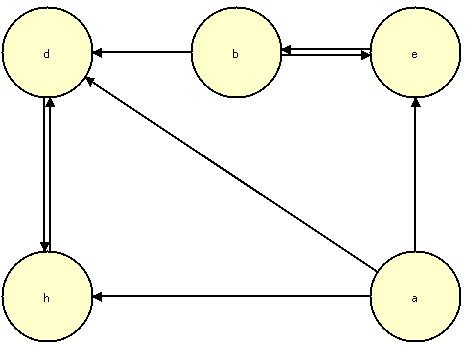
\includegraphics[width=5cm]{figures/GraphDeSurClassement.png}
\caption{Graphe de surclassement}
\end{figure}
\end{multicols}

Avec le seuil de discordance à 0,5, nous pouvons conclure que \textbf{la solution A est la meilleure car elle surclasse les autres et elle n'est pas surclassée} (cf. graphe de surclassement).\\

Cependant, avec le seuil de discordance à 0,3 (donc un peu plus sévère), la solution A semble être à peu près équivalente à la E. En effet, la solution E est assez disparate (certains critères remportent une excellente note, tandis que d’autres critères ont une note très basse), alors que la A est beaucoup plus homogène. Le choix de la meilleure solution entre ces deux-là se fait donc en fonction de notre tolérance à la compensation des notes entre elles.


\begin{appendices} 
\lstlistoflistings

\lstinputlisting[caption=Comptable]{scripts/part1/Comptable.m}
\lstinputlisting[caption=Responsable Atelier]{scripts/part1/ResponsableAtelier.m}
\lstinputlisting[caption=Responsable Commercial]{scripts/part1/ResponsableCommercial.m}
\lstinputlisting[caption=Responsable Stocks]{scripts/part1/ResponsableStock.m}
\lstinputlisting[caption=Responsable Personel]{scripts/part1/ResponsablePersonnel.m}
\newpage
\lstinputlisting[caption=Programation Linéaire Multicritère]{scripts/part2/ad_scores.m}
\lstinputlisting[caption=Programation Linéaire Multicritère]{scripts/part2/gain_matrix.m}
\lstinputlisting[caption=Programation Linéaire Multicritère]{scripts/part2/RepartitionOptimum.m}
\lstinputlisting[caption=Programation Linéaire Multicritère]{scripts/part2/RespEntreprise.m}

\newpage
\lstinputlisting[caption=Analyse Multicritère]{scripts/partie3.m}

\end{appendices} 

%%% End document
\end{document}
